%% Available page modes: oneside, twoside
%% Available languages: english, ngerman
%% Available modes: draft, final (see README)
\documentclass[twoside, english]{thesis}
\addbibresource{thesis.bib}


%% -------------------------------
%% | Custom commands and imports |
%% -------------------------------

\usepackage{xspace}
\usepackage{subcaption}
\usepackage{float}

\renewcommand{\*}{\cdot}
\newcommand{\eps}{\varepsilon}
\newcommand{\bigO}[1]{\ensuremath{\mathcal{O}\!\left(#1\right)}\xspace}

\newcommand{\G}{\ensuremath{G}\xspace}
\newcommand{\E}{\ensuremath{E}\xspace}
\newcommand{\V}{\ensuremath{V}\xspace}
\newcommand{\g}{\ensuremath{g}\xspace}
\newcommand{\e}{\ensuremath{e}\xspace}
\renewcommand{\v}{\ensuremath{v}\xspace}

%% ---------------------------------
%% | Information about the thesis  |
%% ---------------------------------

\author{Samuel Born}
\title{Understanding Small Separators in Road Networks}
\thesistype{Master's Thesis}
%\myinstitute{Institute of Theoretical Informatics}
\grouplogo{scaleLogo}
\reviewerone{m}{T.T.-Prof. Dr. Thomas Bläsius}
\reviewertwo{w}{Dr. Torsten Ueckerdt}
\advisorone{m}{Adrian Feilhauer}
\advisortwo{m}{Michael Z\"undorf}
\editingtime{January 1, 2025}{July 1, 2025}
\settitle


%% ====================================
%% ====================================
%% ||                                ||
%% || Beginning of the main document ||
%% ||                                ||
%% ====================================
%% ====================================
\begin{document}
\pagenumbering{Alph}

%% Set PDF metadata
\setpdf

%% Set the title
\maketitle

%% The Preamble begins here
%% LaTeX2e class for student theses: Declaration of independent work
%% sections/declaration.tex

\thispagestyle{empty}
\null\vfill
\noindent\hbox to \textwidth{\hrulefill} 
%
% Gemäß Studien- und Prüfungsordnung Bachelor Informatik des KIT,
% § 14 (5) vom 10.05.2022
% 
\ifcurrentbaselanguage{English}{I declare that I have developed and written the enclosed thesis completely by myself.
I have not used any other than the aids that I have mentioned.
I have marked all parts of the thesis that I have included from referenced literature, either in their original wording or paraphrasing their contents.
I have followed the by-laws to implement scientific integrity at KIT.}%
{Ich versichere wahrheitsgemäß, die Arbeit selbstständig verfasst, alle benutzten Quellen und Hilfsmittel vollständig und genau angegeben und alles kenntlich gemacht zu haben, was aus Arbeiten anderer unverändert oder mit Abänderungen entnommen wurde sowie die Satzung des KIT zur Sicherung guter wissenschaftlicher Praxis in der jeweils gültigen Fassung beachtet zu haben.}

 
\textbf{Karlsruhe, \theeditend}
\vspace{1.5cm}
 
\dotfill\hspace*{8.0cm}\\
\hspace*{2cm}(\theauthor) 
\cleardoublepage
\frontmatter

%% ----------------
%% |   Abstract   |
%% ----------------

%% For theses written in English, an abstract both in English
%% and German is mandatory.
%%
%% For theses written in German, a German abstract is sufficient.
%%
%% The text is included from the following files:
%% - sections/abstract

\includeabstract

%% ------------------------
%% |   Table of Contents  |
%% ------------------------
\tableofcontents
%\listoffigures
%\listoftables

%% -----------------
%% |   Main part   |
%% -----------------
\mainmatter

%%% LaTeX2e class for student theses
%% sections/evaluation.tex

\chapter{Example}
\label{ch:Example}%anchor point for a reference
In this chapter, we give you some advice for \LaTeX{} and scientific writing to avoid common mistakes.
Most of these rules are just good practice and are not necessarily true in every situation but following them will not hurt you.
You should already be comfortable with \LaTeX{} and Git, take a look at this beginners guide \url{https://www.overleaf.com/learn} if you are not.


\section{Chapters, Sections and Subsections}
\label{sec:Example:Chapters}
Your text should be partitioned by the commands "\texttt{\textbackslash{}chapter}", "\texttt{\textbackslash{}section}", and "\texttt{\textbackslash{}subsection}".
After every headline, there should be some text e.g. a chapter should never begin with a section title.
If you want to reference one part of your text from another part of your text, write something like "see \cref{ch:Example}".
%alternatively use Chapter~\ref{ch:Example}
Take a look at the code to see how to make the number clickable.


\section{Tables}
\label{sec:Example:Tables}
Tables should be \emph{floats} i.e. typeset within "\texttt{\textbackslash{}begin\{table\}}" and "\texttt{\textbackslash{}end\{table\}}" which makes them float to the top of the next page.
Tables should have the full text width.
Further, they should have a meaningful caption placed above them which serves as a standalone explanation and they should also be referenced from the text, like \cref{tb:Example:Tables}.

A visually pleasing table has few lines, unlike tables from e.g. Excel.
A table typically consists of three horizontal lines "$\set{\texttt{top},\texttt{mid},\texttt{bottom}}$\texttt{rule}" and no vertical lines.
Top and bottom rule separate the table from the surrounding text whereas the mid rule separates the header from the data.
All further visual distinction between some rows and columns is achieved by empty space.
For lines, this is possible with the command "\texttt{\textbackslash{}addlinespace}".
The automatic spacing between columns is usually already sufficient.

This example uses the "\texttt{tabularx}" package to make tables.
There are three column types you typically use which are also available in other packages like "\texttt{booktabs}".
Text columns are of type "\texttt{L}" which makes the column left aligned.
Number columns are of type "\texttt{R}" which makes the column right aligned.
Sometimes you use the type "\texttt{C}" to make a column centered.
This is mostly useful for the header row.

\begin{table}[t]
	\caption{This is an example table, the content does not have an actual meaning.
		Note that unlike for figures, the caption is above the content.
		\label{tb:Example:Tables}}
	\begin{tabularx}{\linewidth}{LLRR}
		\toprule
		& Text column & Number column & More numbers \\
		\midrule
		First row & some text & 123\,456 & 1\,234.56 \\
		Second row & some more text & 12\,345\,678 & 7\,839.20 \\
		\addlinespace
		First other row & some text & 654\,321 & 6\,789.10 \\
		Second other row & some more text & 87\,654\,321 & 1\,234.50 \\
		\bottomrule
	\end{tabularx}
\end{table}


\section{Figures}
\label{sec:Example:Figures}
Like tables, Figures should be \emph{floats} i.e. typeset within "\texttt{\textbackslash{}begin\{figure\}}" and "\texttt{\textbackslash{}end\{figure\}}" which makes them float to the top of the next page.
Figures should be centered with "\texttt{\textbackslash{}centering}",
and they should have a meaningful caption which serves as a standalone explanation.
Other than for tables, the cation is placed below the figure.
Further, they should always be referenced from the text, like \cref{fig:Example:figure}.

\begin{figure}[t]
	\centering
	
\includegraphics[height=2.5cm]{logos/kitlogo_en_cmyk.pdf}
	\caption{This is the logo of the KIT and is used as an example image in this work.
	Note that unlike for tables, the caption is below the content.
	\label{fig:Example:figure}}
\end{figure}


\section{Math and Numbers}
\label{sec:Example:MathAndNumbers}
A sentence should always end with a full stop even if the sentence ends with maths like this
\[3987^{12}+4365^{12}=4472^{12}\text{~.}\]
Use the latex command "\texttt{\textbackslash,}" as the thousands separator to make numbers like 12\,345 look nicer.
This is especially useful in tables, see \cref{tb:Example:Tables}.

Math formulas look nicer and are easier to read if you use parentheses of varying sizes, take a look at the following two formulas
\begin{align*}
	f&\in\mathcal{O}((n+m)\cdot\log(n))\\
	g&\in\mathcal{O}\big((n+m)\cdot\log(n)\big)\text{~.}
\end{align*}
Try to avoid starting sentences with a math symbol.
The multiplication symbol is a dot typeset with the command "\texttt{\textbackslash{}cdot}" instead of "$*$" or "$\times$".


\section{Citations}
\label{sec:Example:Citations}
Put citation marks whenever you use statements by another person or published by yourself outside of this work.
Put citation marks at the and of a sentence since they distract the reader.
Dibbelt et al. \cite{DSW16} did something.
Dibbelt et al. did something \cite{DSW16}.


\section{General notes}
\label{sec:Example:Notes}
These are just some unrelated tips and tricks.

\paragraph{Git}
Put every sentence in a new line inside the .tex file to make "\texttt{git diff}" and other commands work nicer.

\paragraph{Text}
Avoid enumeration and itemize environments in written text.
Do not use short forms like "don't".
However, common abbreviations like "et al.", "e.g.", and "i.e." should be used.

\paragraph{Floats}
Try to avoid two floats at the begin of the same page, especially if they are of different types.
See \cref{fig:Example:figure} and \cref{tb:Example:Tables} as a counter example.

\paragraph{TODOs}
As you are working on the document, some things may need further
attention again at a later time.\todo{Include results obtained by
  analyzing the Xen crystal with the anti-mass spectrometer, once the
  experiments are completed.}  Then, it might be useful to annotate
the corresponding part with a \texttt{todo}.  To make it really
obvious that something important is missing at some
point. \todo[inline]{You can include an \texttt{inline} note as well.}
Also do not forget to check your thesis for left-over \texttt{todo}s
before printing and handing in.


\section{Examples}
Some random examples.
\begin{theorem}[Euclid's theorem]
	The set of primes $\mathbb{P}$ is not finite.
	\label{thm:Example:Examples:euclid}
\end{theorem}
\begin{proof}
	Suppose that we have a finite set $\mathbb{P}$ which contains all primes and let $a$ be the product of all primes in $\mathbb{P}$.
	Then $a$ and $a+1$ do not share a common factor other than $1$.
	However, this implies that $a+1$ contains a prime factor which is missing in $\mathbb{P}$.
	Therefore, our assumption that $\mathbb{P}$ contains all primes is wrong which implies that no finite set containing all primes can exist.
\end{proof}

\begin{theorem}
	The set of primes $\mathbb{P}$ is not finite.
\end{theorem}
\begin{proofSketch}
	Take a look at the sum over the inverse of all primes
	\[\sum_{p\in\mathbb{P}} \frac{1}{p}\]
	and show that this sum diverges which directly implies that $\mathbb{P}$ cannot be finite.
\end{proofSketch}

\begin{corollary}
	A direct implication of \cref{thm:Example:Examples:euclid} is that there is no largest prime.
\end{corollary}

\begin{algorithm}[H]
	\Input{An integer $n$.}
	\Output{The largest prime factor of $n$.}
	\BlankLine
	$x \longleftarrow 1$\;
	\ForAll{$i$ \With $i\cdot i \leq n$}{
		\While{$n \bmod i = 0$}{
			$n\longleftarrow \frac{n}{i}$\;
			$x\longleftarrow \max(x, i)$\;
		}
	}
	\If{$n > 1$}{
		$x \longleftarrow n$\;
	}
	\Return{$x$}
	\caption{A factorization algorithm.
	\label{alg:Example:Examples:algorithm}}
\end{algorithm}


\chapter{Introduction}
\label{ch:introduction}

In this chapter, the motivation for this work is explained. 
We shortly introduce our contribution.
Finally, a brief outline of the contents is given.

\section{Motivation}
\label{sec:motivation}

In graph theory, a separator is a subset of vertices whose removal divides the graph into disconnected components of roughly equal size.
The size of these separators significantly affects the performance of numerous algorithms, particularly those utilizing divide-and-conquer approaches.
For instance, Tarjan's and Lipton's foundational work on planar graphs \cite{lipton_applications_1977} demonstrates their utility in optimizing algorithms for many problems like e.g. maximum flow.

Empirical observations from the Customizable Contraction Hierarchies (CCH) paper indicate that road networks may possess remarkably small balanced separators, on the order of \bigO{n^{1/3}} \cite{dibbelt_customizable_2016}.
This finding contrasts with the \bigO{n^{1/2}} separators typical of planar graphs \cite{lipton_separator_1979}, especially since road networks can be considered as nearly planar.
In road networks, these separators enable the creation of effective node orderings, which are critical for the performance of search queries in advanced routing algorithms like CCH.
This thesis seeks to uncover the properties responsible for the presence of such small separators in road networks.
We aim to determine whether these separators stem from inherent graph characteristics, such as limited vertex degrees or sparsity, or from physical real-world features, such as borders, rivers, or a hierachical sturcutre.
Gaining insight into these properties promises to advance our theoretical understanding and offers practical benefits, such as identifying new applications or generating comparable synthetic graphs.
The exploration of small separators in road networks is particularly fascinating due to the rarity of other naturally occurring graph classes exhibiting separators smaller than those in planar graphs.

\section{Contribution}
\label{sec:Contribution}

\todo[inline]{todo}

\section{Outline}
\label{sec:overview}

\todo[inline]{todo}

\chapter{Preliminaries}
\label{ch:Preliminaries}

\section{Graph Theory}
\label{sec:Preliminaries:GraphTheory}

\chapter{Experimental Analysis} \label{ch:experimental_analysis}

\section{Planarity} \label{sec:approach:planarity}

%\todo{mention always intertial flow cutter to compute unless stated otherwise}

Road networks can be modeled as graphs that are nearly planar, meaning they can
be embedded in the plane with only a small number of edge crossings. It is a
well-known result in graph theory that planar graphs admit \(\frac23\)-balanced
separators of size \(\bigO{\sqrt{n}}\), where \(n\) denotes the number of
vertices.

A relevant inquiry is whether the near-planarity of road networks is a critical
feature that influences their structural properties, or if the occasional
non-planar elements are merely incidental and do not substantially affect the
network’s overall characteristics. This prompts the question of how the
separator sizes of road networks are affected when they are transformed into
strictly planar graphs, for instance, by altering edges to eliminate crossings.

To study road networks as planar graphs, we represent roads as linear segments
between points. At each intersection of these segments, a new vertex is
introduced, and the original edges are replaced accordingly. This process
transforms the graph into a planar form by eliminating crossings. For efficient
execution, we utilize a spatial index that stores the bounding boxes of all
edges. Under the assumption of short edges, this structure enables rapid
identification of potential intersections by querying overlapping bounding
boxes, followed by verification of actual crossings. While other algorithms
exist, such as the Bentley-Ottmann algorithm \cite{bentley_algorithms_1979},
which is designed for general segment crossings, or a linear-time algorithm
(e.g., as described in \cite{eppstein_linear-time_2010}), which is tailored for
graph structures with a sublinear number of edge crossings, we opted for this
spatial index-based approach due to its simplicity and ease of implementation,
especially since performance is not a critical concern in this context. Given
that a single edge may intersect multiple times, we sort the intersection
points along each edge and introduce new edges accordingly. Pseudo-code for
this planarization algorithm is provided in \cref{alg:planarization}.

\begin{algorithm}[b]
	\Input{Non-planar graph \(G=(V, E, pos)\).}
	\Output{Planarized version of \G.}
	\BlankLine
	spatial\_index \(\longleftarrow\) load(bounding\_boxes(\E))\;
	crossings \(\longleftarrow\) \{\}\;
	\ForAll{\e  in \E}{
		\ForAll{candidates \(c\) in spatial\_index.query(\e)}{
			\If{\(c\) intersects \e} {
				crossings[\(e\)].append(\(c\))\;
				crossings[\(c\)].append(\(e\))\;
			}
		}
	}
	\ForAll{(\e, crossed) in crossings}{
		\G.remove(\e)\;
		vertices \(\longleftarrow\) get\_intersection\_vertices(\(e\), crossed)\;
		sort vertices along \e\;
		add\_new\_edges(\(e\), vertices)\;
	}
	\caption{Simple planarization algorithm \label{alg:planarization}}
\end{algorithm}

We applied this planarization method to real-world road networks. The Karlsruhe
network, with approximately 120,000 nodes and 150,000 edges, revealed around
2,500 intersections, while the Germany network, comprising about 5.8 million
nodes and 7.2 million edges, exhibited approximately 100,000 intersections.
These figures slightly exceed the \bigO{\sqrt{n}} intersection counts reported
in prior studies but remain within a similar magnitude
\cite{eppstein_linear-time_2010}. These differences could be explained by the
unoptimal linear assumption of edges and might be mitigated by using a more
modeled road network like OpenStreetMap.

Analysis of separator sizes showed minimal variation post-planarization. We
identified \(\frac{2}{3}\)-balanced separators of size approximately
\bigO{n^(1/3)}, aligning with the values from non planar graphs. A comparison of
the separator sizes in the planar and non-planar versions of the Germany
network is depicted in \cref{fig:germany_planar_vs_non_planar}.

\begin{figure}
	\centering
	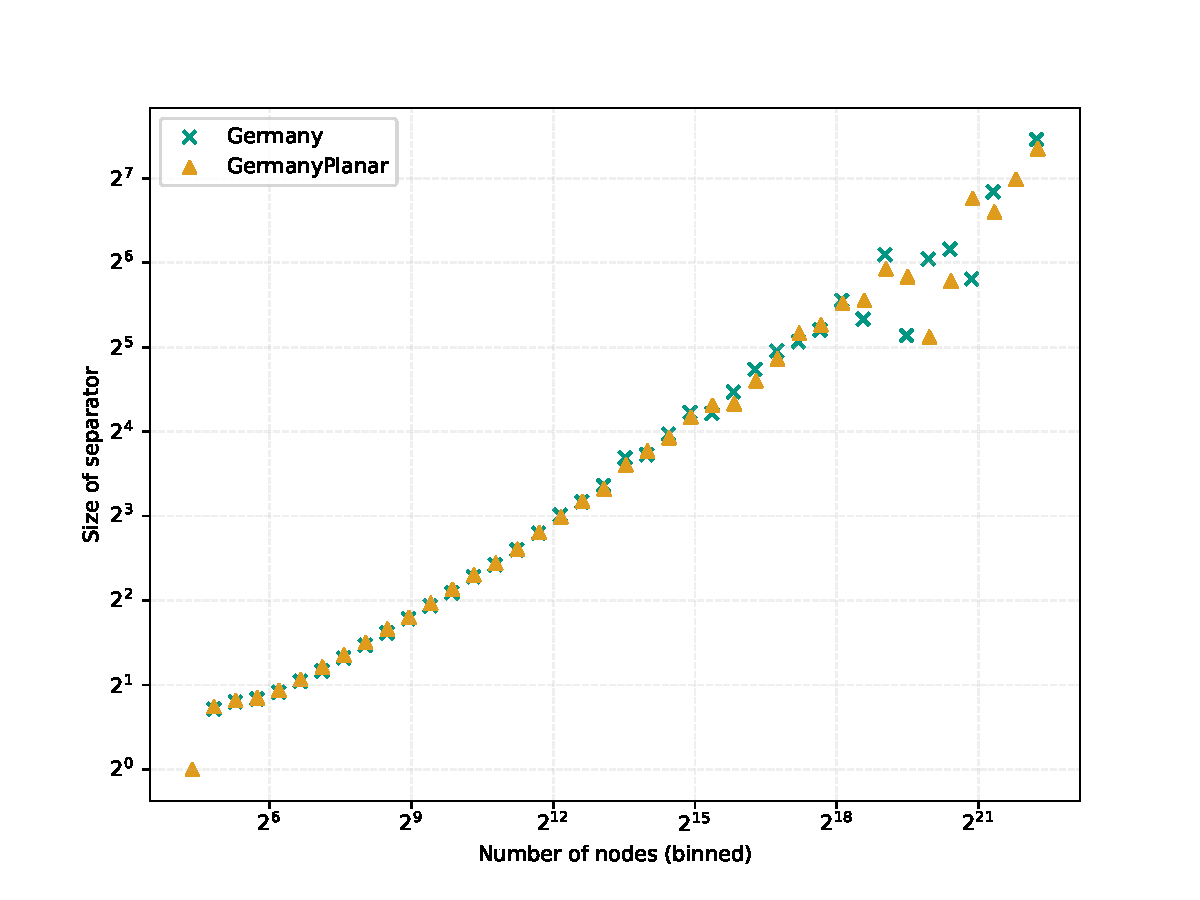
\includegraphics[width=0.8\linewidth]{graphics/GermanyPlanarVsNonPlanar.pdf}
	\caption{Comparison of separator sizes in the German road network: planar vs. non-planar.}
	\label{fig:germany_planar_vs_non_planar}
\end{figure}

Our findings indicate that separators in non-planar road networks closely
resemble those in their planarized versions. Frequently, non-planar separators
are also separators in the planarized graph or can be adapted to planar ones
with the addition of only a few nodes. This can be seen in
\cref{fig:karlsruhe_planar_vs_non_planar}, which depicts a non-planar separator
extended to be a separator in the planarized Karlsruhe network.
\todo{explain they can get larger and smaller}
\todo{also say that separators can increase: simple example two disjoint components that get connected}

\begin{figure}
	\centering
	\begin{subfigure}{0.45\linewidth}
		\centering
		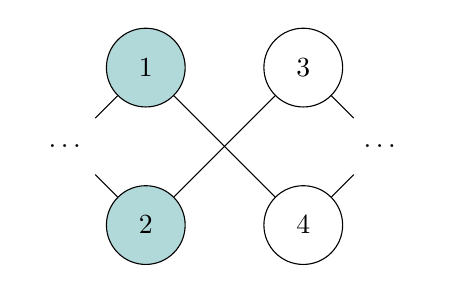
\begin{tikzpicture}[every node/.style={circle, draw, minimum size=1cm}]
			\node[draw=none] (dots1) at (0, 1) {\dots};
			\node[fill=teal!30] (1) at (1, 2) {1};
			\node[fill=teal!30] (2) at (1, 0) {2};
			\node (3) at (3, 2) {3};
			\node (4) at (3, 0) {4};
			\node[draw=none] (dots2) at (4, 1) {\dots};

			\draw (1) -- (4);
			\draw (2) -- (3);

			\draw (1) -- (dots1);
			\draw (2) -- (dots1);
			\draw (3) -- (dots2);
			\draw (4) -- (dots2);
		\end{tikzpicture}
		\caption{Separator in non-planar graph}
	\end{subfigure}
    \hfill
	\begin{subfigure}{0.45\linewidth}
		\centering
		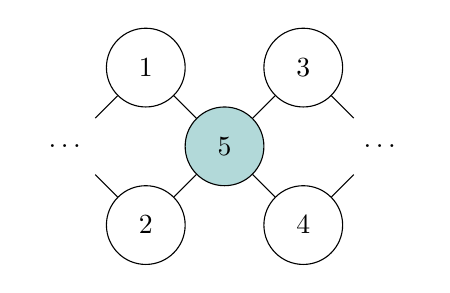
\begin{tikzpicture}[every node/.style={circle, draw, minimum size=1cm}]
			\node[draw=none] (dots1) at (0, 1) {\dots};
			\node (1) at (1, 2) {1};
			\node (2) at (1, 0) {2};
			\node (3) at (3, 2) {3};
			\node (4) at (3, 0) {4};
			\node[fill=teal!30] (5) at (2, 1) {5};
			\node[draw=none] (dots2) at (4, 1) {\dots};

			\draw (1) -- (5);
			\draw (2) -- (5);
			\draw (3) -- (5);
			\draw (4) -- (5);

			\draw (1) -- (dots1);
			\draw (2) -- (dots1);
			\draw (3) -- (dots2);
			\draw (4) -- (dots2);
		\end{tikzpicture}
		\caption{Better separator in planarized graph}
	\end{subfigure}
	\caption{Example of a separator, where a better separator can be found in the planarized graph.}
	\label{fig:planarization_reduces_separator}
\end{figure}

\begin{figure}
	\centering
	\begin{subfigure}{0.45\linewidth}
		\centering
		\begin{tikzpicture}[every node/.style={circle, draw, minimum size=1cm, node distance=1.5cm}]
			\node[fill=teal!30] (1) {1};
			\node[below right=of 1, fill=teal!30] (3) {3};
			\node[left=3cm of 3] (2) {2};
			\node[below left=of 3] (4) {4};

			\draw (1) -- (4);
			\draw (1) -- (2) -- (3);

			\node[right=of 1, draw=none] (dots1) {\dots};
			\node[right=of 4, draw=none] (dots4) {\dots};
			\draw (1) -- (dots1);
			\draw (4) -- (dots4);
			\draw (3) -- (dots4);
			\draw (3) -- (dots1);

			\draw[dashed] (-1, 1) -- (-1, -4.5);
		\end{tikzpicture}
        \caption{Separator in non-planar graph\newline}
	\end{subfigure}
    \hfill
	\begin{subfigure}{0.45\linewidth}
		\centering
		\begin{tikzpicture}[every node/.style={circle, draw, minimum size=1cm, node distance=1.5cm}]
			\node[fill=teal!30] (1) {1};
			\node[below right=of 1, fill=teal!30] (3) {3};
			\node[left=3cm of 3, fill=teal!5] (2) {2};
			\node[below left=of 3, fill=teal!5] (4) {4};
			\node[below= 0.75 of 1, fill=teal!5] (5) {5};

			\draw (1) -- (5);
			\draw (4) -- (5);
			\draw (5) -- (3);
			\draw (1) -- (2) -- (5);

			\node[right=of 1, draw=none] (dots1) {\dots};
			\node[right=of 4, draw=none] (dots4) {\dots};
			\draw (1) -- (dots1);
			\draw (4) -- (dots4);
			\draw (3) -- (dots4);
			\draw (3) -- (dots1);

			\draw[dashed] (-1, 1) -- (-1, -4.5);
		\end{tikzpicture}
        \caption{The separator of the original graph is not a separator in the planarized graph.}
	\end{subfigure}
    \caption{Example where the separator of the original graph is not a separator in the planarized graph.}
\end{figure}



\begin{figure}
	\centering
	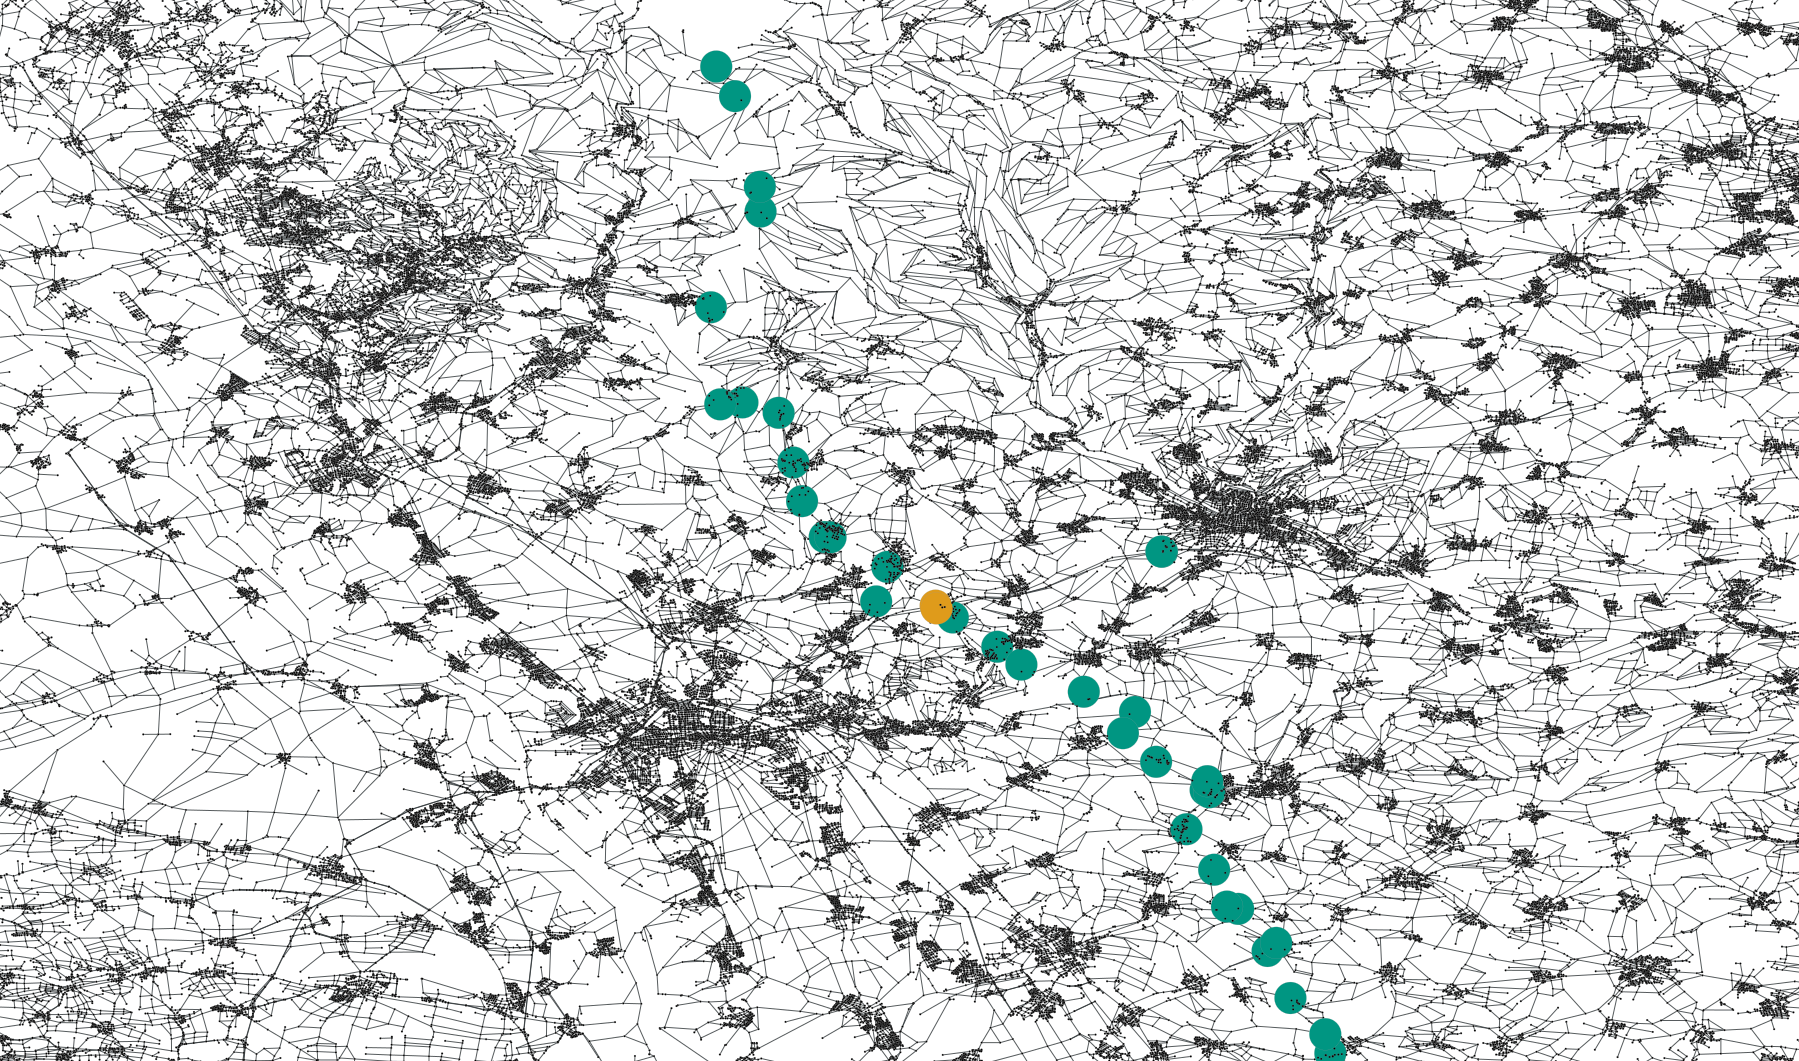
\includegraphics[width=0.8\linewidth]{graphics/karlsruhe_top_level_sep_extended_to_planar_wide.png}
	\caption{Example visualization of one possible top-level separator for
		Karlsruhe. Teal points represent the separator of the original graph, while
		orange points denote the additional nodes required to make it separator
		for the planarized version of Karlsruhe. Separators where computed with
		KaHIP.} \label{fig:karlsruhe_planar_vs_non_planar}
\end{figure}

These findings highlight that the near-planar structure of road networks has
minimal impact on separator size, suggesting that such networks can typically
be analyzed as planar graphs.

\chapter{Evaluation}
\label{ch:evaluation}

\chapter{Conclusion}
\label{ch:conclusion}

This chapter begins by summarizing the key findings, detailing the results of the various models tested.
Subsequently, it addresses the limitations of our experimental approach and outlines several promising directions for future research that build upon the insights gained.

\section{Summary of Findings}
\label{sec:conclusion:summary}

We demonstrate that the separator size of road networks \(s\) scales with graph size \(n\) according to \(\bigO{n^{0.37}}\).
This exponent is slightly larger than the previously suggested \(\bigO{n^{1/3}}\) \cite{dibbelt_customizable_2016} but remains substantially better than the \(\bigO{n^{1/2}}\) bound for planar graphs.

Our investigation systematically demonstrates the insufficiency of simple, isolated graph properties to explain this behavior.
Models based solely on degree distribution or basic geometric locality consistently produce separators that scale as \bigO{n} or \bigO{n^{1/2}}.
Even considering graphs with a geometric embedding, which is defining feature of road networks, standard models like grids or Delaunay triangulations fail to reproduce the target scaling.
Furthermore, planarizing real road networks has a negligible impact on their separator sizes, suggesting that the non-planarity of these graphs is not a primary factor in the observed small separators.

In contrast, models incorporating a hierarchical structure show significant promise.
Our proposed hierarchical Delaunay generator constitutes an entire parameterized class of graphs.
By carefully tuning its parameters, which govern expansion fractions, points per site, and radii across multiple levels, this model is also capable of replicating the observed \bigO{n^{0.37}} scaling.
Notably, the resulting graph structures often bear a strong visual resemblance to those generated by the physical barrier model.

The most successful synthetic model developed in this thesis, however, is one based on simulating physical barriers using multi-scale Perlin noise.
This approach generates a layered landscape of obstacles at various scales, constraining where vertices can be placed.
Remarkably, graphs generated using this method, which combines noise-based point sampling and a Delaunay triangulation, naturally produce separators that scale approximately as \bigO{n^{0.37}}.
An optional pruning step can be employed to reduce the average degree, but this is not strictly necessary to achieve the desired scaling.
This result is achieved without extensive parameter fine-tuning, suggesting that this model captures a more fundamental generative principle.
Ablation studies further underscore this finding, demonstrating that the full spectrum of noise scales, from large, regional barriers to small, local ones, is crucial for achieving this specific scaling across a wide range of graph sizes.

It is important to qualify, however, that the need for a multi-scale or hierarchical structure is not strictly necessary if one allows for extreme parameter fine-tuning.
The tree-locality model, for instance, could replicate the desired scaling using a highly specific distance-decay function \(f(\text{dist}) = 1/\text{dist}^{3.3}\).
This case serves as an interesting exception, highlighting that specific correlation structures can be enforced without an explicit hierarchy, though this offers less insight into the natural emergence of such properties.

Revisiting the central research question, \enquote{Do small separators in road networks arise from intrinsic graph properties, or from real-world physical barriers?}, our findings provide a nuanced answer.
The evidence strongly suggests that small separators are not a consequence of any single, simple graph property but are an emergent feature of a multi-scale structural organization.
This multi-scale structure can be interpreted as an explicit hierarchy of road types or, perhaps more fundamentally, as the result of physical barriers existing at all geographic scales.
The success of the multi-scale Perlin noise model indicates that the constrained placement of nodes by geography is a powerful generative mechanism.
Road networks are built upon a landscape permeated by obstacles at every scale, from mountain ranges down to local properties.
This forces the graph to be composed of densely connected regions that are themselves sparsely interconnected through well-defined corridors, a structure highly amenable to small separators.
Therefore, we conclude that the small separators in road networks are a direct result of their adaptation to a multi-scale, obstacle-rich environment.

\section{Limitations and Future Work}
\label{sec:conclusion:future_work}

The conclusions presented in this thesis are primarily derived from experimental analysis.
While our results strongly indicate the importance of hierarchy and multi-scale barriers, the inability of simpler, non-hierarchical models to reproduce the desired scaling does not constitute a formal disproof of their potential under different assumptions.
A notable limitation is that our most successful models rely on a final Delaunay triangulation.
The observation that k-Nearest Neighbor graphs built on the same hierarchical point sets fail to produce the correct scaling suggests that the specific connectivity pattern of Delaunay graphs, which allows for both local and some structured long-range connections, plays a significant, yet not fully explored, role.

These limitations and findings open several avenues for future research.
A primary direction is the pursuit of a rigorous theoretical analysis of the multiplicative Perlin noise model.
Such a study could potentially provide a formal derivation for the empirically observed \bigO{n^{0.37}} scaling.
Further work could also seek to improve the efficiency of the generative algorithms.
For instance, the tree-locality generator is hampered by its slow, BFS-based distance calculations; developing an efficient method to sample edges according to weights derived from tree distances would make this model more viable for large-scale tests.
The synthetic generators developed here can serve as a basis for creating realistic, large-scale benchmarks for evaluating not only route planning algorithms but also other algorithms that depend on graphs with small separators.
An important extension of this work would be to adapt the noise generation algorithm to more closely replicate other key road network metrics beyond just separators, such as hop distributions, to create an even more robust synthetic road network generator.



%% --------------------
%% |   Bibliography   |
%% --------------------
%% Add entry to the table of contents for the bibliography
\printbibliography[heading=bibintoc]

%% ----------------
%% |   Appendix   |
%% ----------------
%\appendix
%%% LaTeX2e class for student theses
%% sections/apendix.tex

\iflanguage{english}
{\chapter{Appendix}}    % english style
{\chapter{Anhang}}      % german style
\label{chap:appendix}


%% -------------------
%% | Example content |
%% -------------------
\section{First Appendix Section}
\label{sec:appendix:FirstSection}
		
\setcounter{figure}{0}
		
\begin{figure} [ht]
  \centering
  \caption{A figure}
  \label{fig:anotherfigure}
\end{figure}
\dots


\end{document}
